\documentclass{beamer}
%\usepackage [russian]{babel}
\usepackage [english]{babel}
\usepackage {amssymb}
\usepackage {amsmath}
%\usepackage {beamerthemeBerlin}
\usetheme{Darmstadt}
%\usetheme{Warsaw}
\title{Theory of shadowing and its applications.}
\author{
Alexey V. Osipov\inst{1}\ %\and Sergei Yu. Pilyugin\inst{1}\and Sergei~B.~Tikhomirov\inst{2}
%\\
%{\small{Joined research with Sergei Yu. Pilyugin\inst{1} and Sergei~B.~Tikhomirov\inst{2}.}}
}
\institute{
\inst{1}
Chebyshev Lab of Saint-Petersbourg State University
%\and
%\inst{2}
%National Taiwan University
}
\date{May 2011}
\begin{document}
\begin{frame}
%\maketitle
\titlepage
\end{frame}
\begin{section}{Definitions}
\begin{frame}{$d$-pseudotrajectory}
\begin{itemize}
	\item $M$ manifold, dist, $f\in\mbox{Diff}^1(M)$, $O(p,f)=\{f^n(p)\}_{n\in\mathbb{Z}}$
  \item $\xi=\{x_n\}$ is a $d$-pseudotrajectory, if 
	$$\mbox{dist}(x_{n+1},f(x_n))\leq d\quad \forall n\in\mathbb{Z}.$$
\begin{figure}
	\centering
	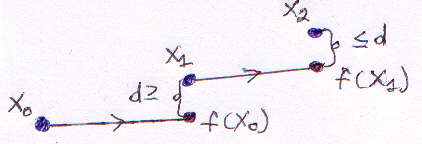
\includegraphics{scan1.jpg}
\end{figure}	
\end{itemize}
\end{frame}
\begin{frame}{POTP}
\begin{itemize}
\item $\forall\epsilon>0\ \exists d>0$ such that $\forall d$-pseudotrajectory $\xi$ there exists an exact trajectory $\{p_n = f^n(p)\}$ such that
$$\mbox{dist}(x_n,p_n)<\epsilon\quad \forall n\in\mathbb{Z}.$$
\begin{figure}
	\centering
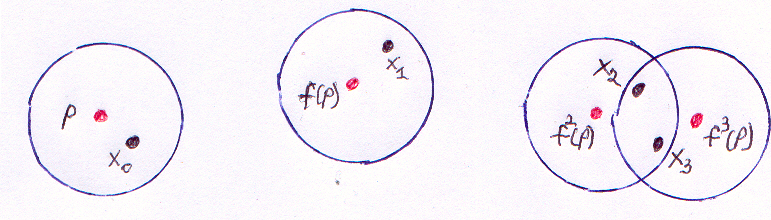
\includegraphics[scale=0.5]{scan2.jpg}
\end{figure}
\item Example, where POTP holds:

\begin{figure}
	\centering
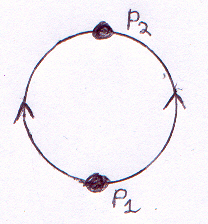
\includegraphics[scale=0.5]{scan3.jpg}
\end{figure}
\end{itemize}
\end{frame}

\begin{frame}{OSP and WSP}
\begin{itemize}
\item
$f\in\mbox{OSP} \Leftrightarrow$
$\forall\epsilon>0\ \exists d>0$ such that $\forall d$-pseudotrajectory $\xi$ there exists an exact trajectory $O(p,f)$ of a point $p$ such that
$$\xi\subset N(\epsilon,O(p,f))\quad\mbox{and}\quad O(p,f)\subset N(\epsilon,\xi).$$ 
\item Example where OSP holds and POTP does not hold:

%\begin{center}
an irrational rotation of the circle $$x\mapsto g(x)=x+\alpha\quad\mbox{for }\alpha\notin\mathbb{Q}.$$
%\end{center}
\item
$f\in\mbox{WSP} \Leftrightarrow$
$\forall\epsilon>0\ \exists d>0$ such that $\forall d$-pseudotrajectory $\xi$ there exists an exact trajectory $O(p,f)$ of a point $p$ such that
$$\xi\subset N(\epsilon,O(p,f)).$$ 
\end{itemize}
\end{frame}
\end{section}
\begin{section}{Main problems}
\begin{frame}{Main problems}
\begin{itemize}
  \item $H(M)$ with $C^0$-metric, $\mbox{Diff}^1(M)$ with $C^1$-metric

  \item a set is \textbf{generic} if it contains a countable intersection of open and dense sets 

	\item[(P1)] Is the set of mappings having some shadowing property generic in Baire sense (for space $H(M)$, $\mbox{Diff}^1(M)$)? 
	
	\item[(P2)] Characterisation of sets of diffeomorphisms having some shadowing property in terms of hyperbolic theory.
\end{itemize}
\end{frame}
\end{section}

\begin{section}{Genericity problem}
\begin{frame}{Results}
\begin{figure}
	\centering
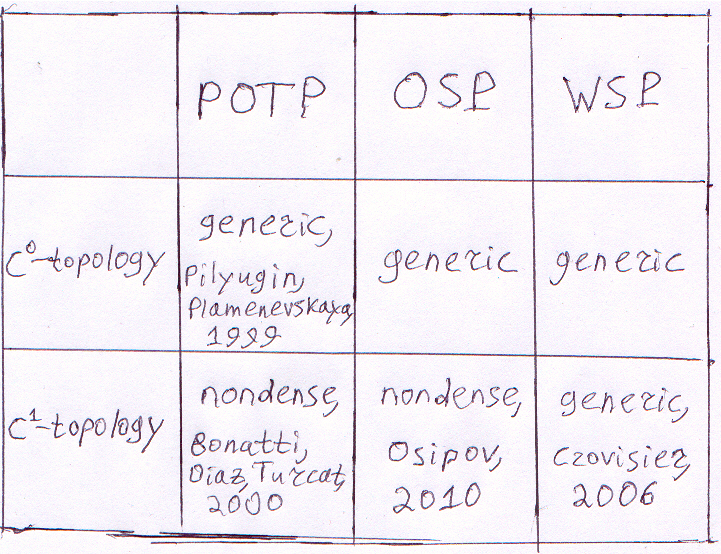
\includegraphics[scale=0.7]{scan4.jpg}
\end{figure}
\end{frame}

\begin{frame}{Hyperbolic set, definition.}

$A$ is a \textbf{hyperbolic set} for $f\in\mbox{Diff}^1(M)$ $\Leftrightarrow$ \\ 
\ \ \ \ \ $A$ is a compact $f$-invariant set and \\
\ \ \ \ \ there exist constants $C$ and $\lambda$ such that\\
\ \ \ \ \  for all $p\in A$ there exist complementary linear subspaces\\
\ \ \ \ \ $E^s(p)$ and $E^u(p)$ of $T_p M$ and

$$|Df^k(p)v|\leq C\lambda^k|v|,\quad\forall v\in E^s(p), k\geq 0,$$ 
$$|Df^{-k}(p)v|\leq C\lambda^k|v|,\quad\forall v\in E^u(p), k\geq 0.$$
\end{frame}
\begin{frame}{Hyperbolic set, stable and unstable manifolds.}
\begin{itemize}
\item If $A$ is a hyperbolic set then $\forall p\in A$ there exist 
manifolds $W^s(p)$ and $W^u(p)$ (stable and unstable manifolds) such that
$$\mbox{dim} W^s(p) = s,\quad\mbox{dim} W^u(p) = u,$$
%$$\forall x\in W^s(p), y\in W^u(p)\quad f^n(x)\rightarrow p,\quad f^n(y)\rightarrow\quad\mbox{as }n\rightarrow+\infty.$$
$$f^n(x)\longrightarrow p,\quad\mbox{as }n\rightarrow+\infty \qquad \forall x\in W^s(p),$$
$$f^{-n}(x)\longrightarrow p,\quad\mbox{as }n\rightarrow+\infty \qquad \forall x\in W^u(p).$$
\item The number $u$ is called an \textbf{index} of a hyperbolic set $A$.
\item Hyperbolic periodic point.
\end{itemize}
\end{frame}

\begin{frame}{$C^1$-nondensity of POTP}
DA-diffeomorphism of Williams on $\mathbb{T}^2$:

\begin{figure}
	\centering
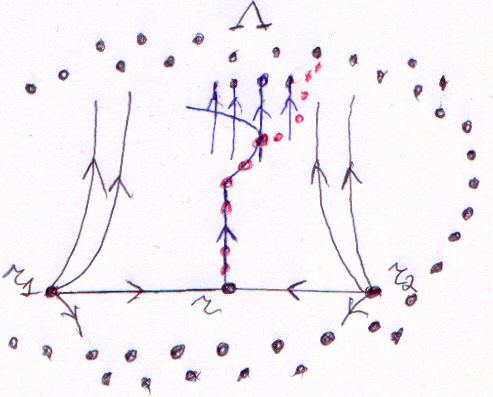
\includegraphics[scale=0.5]{scan5.jpg}
\end{figure}

$r_1,r_2$ are hyperbolic repellers, $r$ --- saddle, $\Lambda$ --- hyperbolic attractor.
\end{frame}
\begin{frame}{$C^1$-nondensity of OSP}

Example of Ilyashenko and Gorodetski: domain $W\subset\mbox{Diff}^1(S^2\times S^1)$

\begin{itemize}
	\item partially hyperbolic set $S$ homeomorphic to the product of a Cantor set and a circle
	
	\begin{figure}
	\centering
	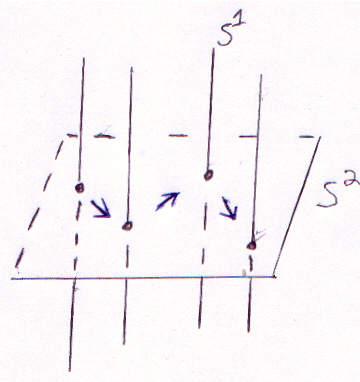
\includegraphics[scale=0.6]{scan6.jpg}
	\end{figure}
	
	\item hyperbolic points with different indices are dense in $S$
\end{itemize}
\end{frame}
\begin{frame}{$C^1$-nondensity of OSP, case (A1)}
There exist two hyperbolic periodic points $r_1$ and $r_2$ with $\mbox{dim}(W^s(r_1))=2=\mbox{dim}(W^u(r_2))$ and $\mbox{dim}(W^u(r_1))=1=\mbox{dim}(W^s(r_2))$ such that $$W^u(r_1)\cap W_s(r_2)\neq\emptyset.$$

\begin{figure}
	\centering
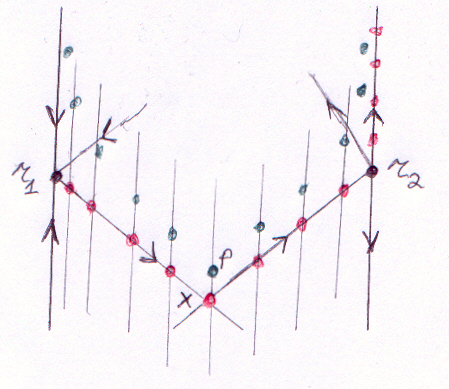
\includegraphics[scale=0.5]{scan7.jpg}
\end{figure}
\end{frame}
\begin{frame}{$C^1$-nondensity of OSP, case (A2)}

Not case (A1). Fix hyperbolic periodic points $r_1,\ldots,r_4$ such that 
$$\mbox{dim} W^u(r_1)=\mbox{dim} W^u(r_2)=1,\quad \mbox{dim} W^s(r_3)=\mbox{dim} W^s(r_4)=1.$$

\begin{figure}
	\centering
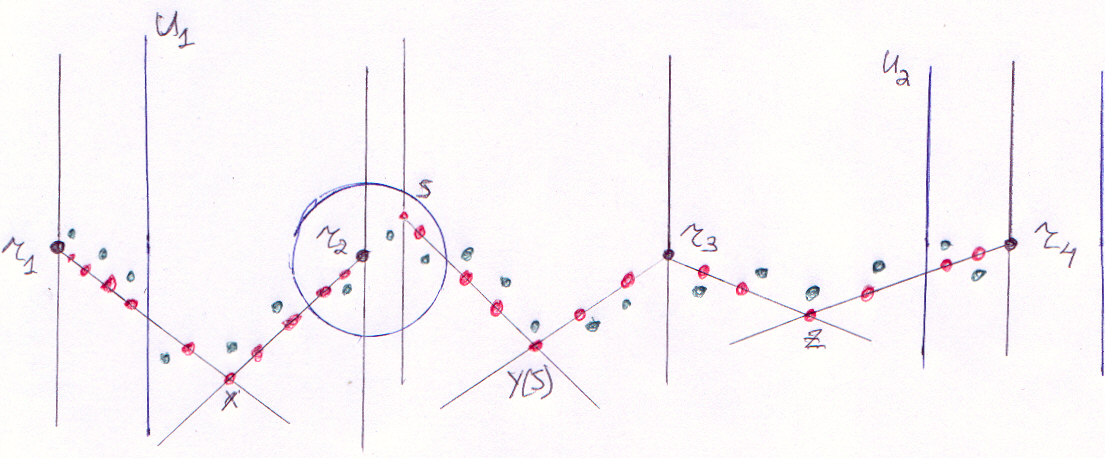
\includegraphics[scale=0.5]{scan8.jpg}
\end{figure}
\end{frame}
\end{section}

%$\mbox{dim}W^u(s)=2,\quad\mbox{dim}W^u(s)=1.$

\begin{section}{Characterisation problem}
\begin{frame}{Nonwandering set}
\begin{itemize}
	 \item A point $p$ is wandering for $f$ if $\exists U\ni p$ such that $f^{n}(U)\cap U =\emptyset$ for all $n$ with sufficiently large $|n|$.  
   \item Alternative definition: a point p is nonwandering for $f$ if
   $\exists\{p_k\}_{k\geq0},\{n_k\}_{k\geq0}$ such that $n_k\rightarrow\infty$ and
   $$p_k\rightarrow p,\quad f^{n_k}(p_k)\rightarrow p.$$
\end{itemize}
\end{frame}
\begin{frame}{Structural stability}
\begin{itemize}
	\item $f\in\mathbb{S}$ $\Leftrightarrow$ %$f$ is topologically conjugate with any diffeomorphism from its small neighborhood
	$\exists U$ such that $\forall g\in U$ $\exists h\in H(M)$ such that $hf=gh$. 
	\item (Robbin,Robinson,$Ma\tilde{n}\acute{e}$, 1988) \textbf{structural stability} is equivalent to \textbf{Axiom A}
	(the nonwandering set is hyperbolic and is the closure of periodic points)
	 and \textbf{strong transversality condition}
	 \item 	Spectral decomposition theorem (Smale): Axiom A implies
	
	$\Omega(f)=\Omega_1\cup\ldots\cup\Omega_m$, $\Omega_j$ is hyperbolic and has a dense semi-trajectory.

\end{itemize}
\end{frame}	 
\begin{frame}{$\Omega$-stability}
\begin{itemize}
%	\item $q$ is a nonwandering point for $f$ if $\exists U(f)$ such that for any number $N$
  \item $f\in\Omega\mathbb{S}$ $\Leftrightarrow$ $f$ and any diffeomorphism from its small neighborhood are topologically conjugate on nonwandering sets
  \item (Palis, 1987) $\Omega$\textbf{-stability} is equivalent to \textbf{Axiom A} and \textbf{no cycle condition} 
  
  \begin{figure}
	\centering
  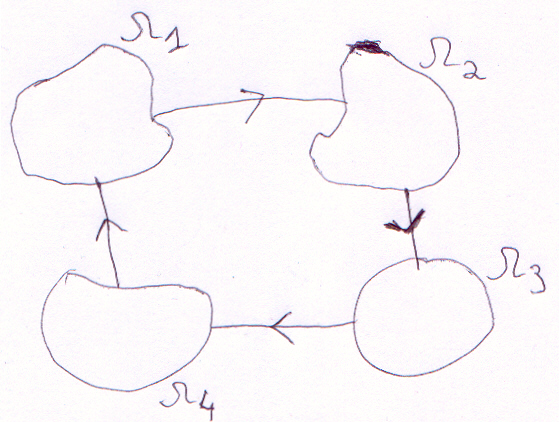
\includegraphics[scale=0.5]{scan9.jpg}
  \end{figure}
\end{itemize}
\end{frame}
\begin{frame}{Results}
\begin{itemize}
\item $$\mbox{POTP}\neq\mathbb{S},$$ $$\mbox{Int}^1(\mbox{POTP}) = \mbox{Int}^1(\mbox{OSP}) = \mathbb{S},$$ %$$\mbox{Int}^1(\mbox{WSP})\neq \Omega\mathbb{S};$$
\item \textbf{LipSP, Lipschitz shadowing:} (POTP with $\epsilon=Ld$) $\exists L,d_0 $ such that for any $d$-pseudotrajectory $\xi$ with $d\leq d_0$ there exists a point $p$ such that
$$\mbox{dist}(x_k,f^k(p))\leq Ld\quad\forall k\in\mathbb{Z}.$$
\item (Pilyugin, Tikhomirov, 2010) $\mbox{LipSP} = \mathbb{S}$. 
\end{itemize}
\end{frame}
\begin{frame}{Periodic shadowing}
\begin{itemize}
	\item \textbf{Periodic shadowing} (PerSh)
	
		$\forall\epsilon>0\ \exists d>0$ such that $\forall$ periodic $d$-pseudotrajectory $\xi$ there exists a periodic exact trajectory $\{p_n\}$ such that
	$$\mbox{dist}(x_n,p_n)<\epsilon\quad \forall n\in\mathbb{Z}.$$
	\item \textbf{Lipschitz periodic shadowing} (LipPerSh)
	
	PerSh with $\epsilon=Ld$.
	\item (Pilyugin, Tikhomirov, Osipov, 2010) $$\mbox{Int}^1(\mbox{PerSh})=\mbox{LipPerSh} = \Omega \mathbb{S}.$$
\end{itemize}	
\end{frame}
\begin{frame}{General Scheme of the Proof}
\begin{itemize}
%	\item $\Omega \mathbb{S}\subset \mbox{LipPerSh}$
%	\item $\mbox{Int}^1(\mbox{PerSh})\subset\Omega \mathbb{S}$ \\
%	(using result of Hayashi and Aoki: $\mbox{Int}^1(HP)=\Omega\mathbb{S}$, 
%	where HP is the set of diffeomorphisms whose periodic points are hyperbolic)
%	\item $f\in\mbox{LipPerSh}\Rightarrow f\in\Omega \mathbb{S}$
%\begin{itemize}
%	\item Step 1. hyperbolicity of periodic points
%	\item Step 2. uniform hyperbolicity of periodic points
%	\item Step 3. $f$ has the Axiom A
%	\item Step 4. $f$ satisfies the no-cycle condition
%\end{itemize}
	\item $\Omega S\subset \mbox{LipPerSh}$
	\item $\mbox{Int}^1(\mbox{PerSh})\subset\Omega S$
	\item $f\in\mbox{LipPerSh}\Rightarrow f\in\Omega S$
\begin{itemize}
	\item Step 1. hyperbolicity of periodic points
	\item Step 2. uniform hyperbolicity of periodic points
	\item Step 3. $f$ has the Axiom A
	\item Step 4. $f$ satisfies the no-cycle condition
\end{itemize}
\end{itemize}
\end{frame}
\begin{frame}{Proof of $\Omega S\subset\mbox{LipPerSh}$}
\begin{itemize}
%	\item Expansivity
%	
%	$\exists a>0$ such that if $\mbox{dist}(f^n(x),f^n(y))<a$ $\forall n\in\mathbb{Z}$ then $x=y$
	\item Spectral decomposition theorem: 
	
	$\Omega(f)=\Omega_1\cup\ldots\cup\Omega_m$, $\Omega_j$ is hyperbolic and has a dense semi-trajectory
  \item $\xi$ is a periodic $d$-pseudotrajectory, $\xi\subset U(\Omega_j)$ for some $j$ 
	\item Shadowing lemma: 
	
	if $\Lambda$ is hyperbolic then $f$ has LipSh and is expansive in some~$U(\Lambda)$
	\item Expansivity means that a $d$-pseudotrajectory can be shadowed only by one $p$ 
\end{itemize}
%\end{block}
\end{frame}
%\end{section}
%\begin{section}{Proof of $\mbox{Int}^1(\mbox{PerSh})\subset\Omega S$}
\begin{frame}{Proof of $\mbox{Int}^1(\mbox{PerSh})\subset\Omega S$}
%\begin{block}
\begin{itemize}
	\item HP --- set of diffeomorphisms $f$ such that every periodic point of $f$ is hyperbolic
	
	Lemma (Aoki, 1992, Hayashi, 1992). $\mbox{Int}^1(\mbox{HP})=\Omega S$
	\item It is enough to prove that $\mbox{Int}^1(\mbox{PerSh})\subset\mbox{HP}$
	%\item $\forall x\in M$ $\exp_x$ and $\exp_x^{-1}$ are locally Lipschitz with constant $2$
	\item %Let $f\in\mbox{Int}^1(\mbox{PerSh})\backslash\mbox{HP}$ with nonhyperbolic fixed $p$ and an eigenvalue $\lambda=1$. Let $h$ be a $C^1$-small pertubation of $f$ such that for $H:=\exp_p^{-1}\circ h\circ\exp_p$ the following holds
	%$$H(u,w)=(u,Bw).$$ 
	$h$ is a $C^1$-small pertubation of $f$ that is linear in $U(p)$, $p$ is a nonhyperbolic periodic point for $h$
\end{itemize}
\end{frame}
%\end{section}
%\begin{section}{Proof of $\mbox{LipPerSh}\subset\Omega S$}
\begin{frame}{Proof of $\mbox{LipPerSh}\subset\Omega S$, Steps 1 and 2}
\begin{itemize}
\item $f, f^{-1}\in\mbox{LipPerSh}$ with $L>1$
\item Lemma: Every periodic point is hyperbolic
%\begin{itemize}
%	\item $f$ has a nonhyperbolic fixed point $p$ with an eigenvalue $\lambda=1$. 
%	$$F(v)=\exp_p^{-1}\circ f\circ\exp_p(v)=Av+\phi(v)$$
%	There exist coordinates $v$ such that
%	$$A=DF(p)=\mbox{diag}(B,P),\quad
%	B=
%	\left(\begin{matrix}
%	1&1\\
%	0&1
%	\end{matrix}
%	\right)
%	$$ 
%	\item $y_K=(Z_1(K)d,Kd,0,\ldots,0),\quad y_{2K}=(Z_2(K)d,0,0,\ldots,0)$
%	\item $Q=2K+Z_2(K)$, $y_Q=y_0=0$
%	\item $\xi=\{x_k=\exp_p(y_k)\}$ is a $Q$-periodic $4d$-pseudotrajectory
%\end{itemize}
%\end{itemize}
\item Key lemma: Set of all periodic points of $f$ has all properties of a standard hyperbolic set except compactness.
$$|Df^j(p)v_s|\leq C\lambda^j|v_s|,\quad |Df^{-j}(p)v_u|\leq C\lambda^j|v_u|,$$ where $j\geq0$, $v_s\in S(p)$, $v_u\in U(p)$
\begin{itemize}
\item $p$ is an $m$-periodic point, let $v_0=v_u\in U(p)$, $v_{i+1}=Df^i(p)v_i$, 
$$\lambda_i=|v_{i+1}|/|v_i|,\quad 	a_0=\tau,\ \  a_{i+1}=\lambda_i a_i-1,$$ %where $\tau$ depends only on $\lambda_j$ for $0\leq j\leq m-1$
where $\tau$ is chosen such that $a_m=0$ 
	\item $w_i=a_iv_i/|v_i|$ for $0\leq i\leq m-1$, $\{w_i\}$ is an $m(n+1)$-periodic%, $w_m=B^{-n}\tau v_0/|v_0|$, $w_{m+1+i}=A_iw_{m+i}$ for $0\leq i\leq mn-1$, where $n=\dim M$,
	%$w_{km}=B^{k-1-n}\tau|v_0|/|v_0|$ for $1\leq k\leq n+1$
	\item $|Df^i(p)v_u|=\lambda_0\cdot\ldots\lambda_{i-1}>\frac{1}{16L}\left(1+\frac{1}{8L}\right)^i|v_u|, \quad 0\leq i\leq m-1.$
\end{itemize}
\end{itemize}
\end{frame}
%\begin{frame}{Proof of $\mbox{LipPerSh}\subset\Omega S$, Part 4}
%\begin{itemize}%
%	\item sequence $\xi=\{x_i=\exp_{p_i}(dw_i)\}$ is an $m(n+1)$-periodic $4d$-pseudotrajectory 
%	\item inequality $\mbox{dist}(x_i,f^i(p))\leq 4Ld$ implies relation $|a_i|\leq 8Ld$ for $0\leq i\leq m-1$,
%	\item Remind that $\lambda_i=(a_{i+1}+1)/a_i$, $\lambda_i=|Df^{i+1}(p)v_u|/|Df^i(p)v_u|$
%	\item
%	$$|Df^i(p)v_u|=\lambda_0\cdot\ldots\lambda_{i-1}=$$
%	$$=\frac{a_{i}+1}{a_0}\left(1+\frac{1}{a_1}\right)\ldots\left(1+\frac{1}{a_{i-1}}\right)>$$
%	$$> \frac{1}{16L}\left(1+\frac{1}{8L}\right)^i|v_u|, \quad 0\leq i\leq m-1.$$
%\end{itemize}
%\end{frame}
\begin{frame}{Proof of $\mbox{LipPerSh}\subset\Omega S$, Steps 3 and 4}
\begin{itemize}
	\item Lemma: $f$ satisfies the Axiom A
\begin{itemize}
  \item $P_l$ --- the set of periodic points of index $l$
	\item $\mbox{Cl}P_l$ is a hyperbolic set.
	\item density of periodic points in $\Omega(f)$
\end{itemize}
	\item Lemma:	$f$ has no cycles 
\begin{itemize}
\item any cycle is approximated by periodic pseudotrajectories
\item any cycle is approximated by periodic exact trajectories
\item \ 
\begin{figure}
	\centering
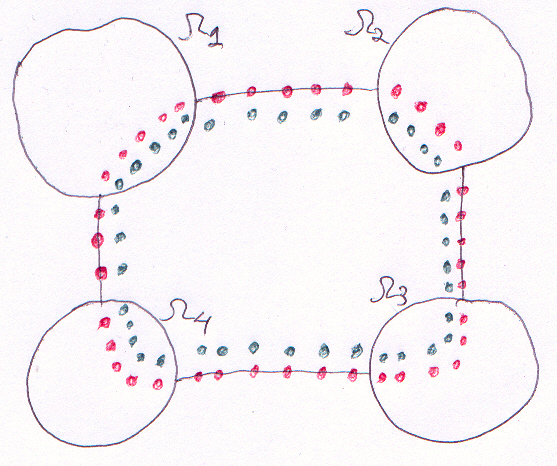
\includegraphics[scale=0.4]{scan10.jpg}
\end{figure}
%	\item For simplicity we prove that $f$ has no $1$-cycles. Suppose there exists $p\in (W^u(\Omega_i)\cap W^s(\Omega_i))\backslash\Omega(f)$.
%	\item construct a periodic $d$-pseudotrajectory coming through $p$ and ''cycling'' around $\Omega_i$
%	\item $p$ is a limit of periodic points 
\end{itemize}
\end{itemize}
\end{frame}
\begin{frame}{Inverse shadowing}
\begin{itemize}
\item A $d$\textbf{-pseudomethod} is a sequence of continuous mappings $\{\Psi_k\}_{k\in\mathbb{Z}}$ such that 
$$\mbox{dist}(\Psi_k(x),f(x))\leq d\quad\forall k\in\mathbb{Z}.$$
\item We say that a sequence $\{x_k\}$ is \textbf{a pseudotrajectory generated by a }$d$\textbf{-pseudomethod} $\{\Psi_k\}_{k\in\mathbb{Z}}$ if
$$x_{k+1} = \Psi_k(x_k)\quad\forall k\in\mathbb{Z}.$$ 
\item $f\in\mbox{InvSh}$ $\Leftrightarrow$ $\forall\epsilon>0\ \exists d>0$ such that for any point $p$ and for any $d$-pseudomethod $\{\Psi_k\}_{k\in\mathbb{Z}}$ there exists a pseudotrajectory $\{x_k\}$ generated by this method such that
$$\mbox{dist}(x_k,f^k(p)) < \epsilon,\quad \forall k\in\mathbb{Z}.$$

\end{itemize}
\end{frame}
\begin{frame}{Inverse periodic shadowing}
\begin{itemize}
\item $\mbox{Int}^1(\mbox{InvSh})=\mbox{LipInvSh}=\mathbb{S}$.
\item 
Inverse periodic shadowing (InvPerSh) = inverse shadowing for periodic points.
%$f\in\mbox{InvPerSh}$ $\Leftrightarrow$ $\forall\epsilon>0\ \exists d>0$ such that for any periodic point $p$ and for any $d$-pseudomethod $\xi$ there exists a pseudotrajectory $\{x_k\}$ generated by this method such that
%$$\mbox{dist}(x_k,f^k(p)) < \epsilon,\quad \forall k\in\mathbb{Z}.$$
\item LipInvPerSh:        

InvPerSh with $\epsilon=Ld$.
\item

Theorem: 

1) $\mbox{Int}^1(\mbox{InvPerSh}) = \Omega \mathbb{S}$,

2) LipInvPerSh is equivalent to hyperbolicity of $Cl(Per(f))$.

%%%Tell them that it is the same, but different

\end{itemize}
\end{frame}
\end{section}
\begin{section}{Shadowing for flows}
\begin{frame}{Shadowing for flows}
%%%this property is almost the same with standard shadowing property for flows
\begin{itemize}
  \item $\Phi$ is the flow, $\Phi:\mathbb{R}\times M\mapsto M$
	\item \textbf{standard shadowing:} $\forall \epsilon>0$ $\exists d>0$ %and $\{d_k\}\leq d$ 
	such that for any increasing $\{\Delta_k\}_{k\in\mathbb{Z}}$ such that
$$|\Delta_{k+1} - \Delta_k|\leq 1\ \forall k\in\mathbb{Z},\quad \lim{\Delta_k}=\infty\mbox{ for }k\rightarrow\infty$$	
	 $\forall\{x_k\}_{k\in\mathbb{Z}}$ such that
	$$|x_{k+1} - \Phi(\Delta_{k+1} - \Delta_k, x_k)|\leq d\quad\forall k\in\mathbb{Z}$$
	$\exists p$ and $\exists \{t_k\}$ such that 
	$$|x_k - \Phi(t_k,p)|\leq\epsilon\quad\forall k\in\mathbb{Z}$$
	$$\mbox{and }|(\Delta_{k+1} - \Delta_k) - (t_{k+1} - t_k)|\leq\epsilon.$$
	\item for \textbf{oriented shadowing} the last condition is changed to
   $$(\Delta_{k+1} - \Delta_k)/(t_{k+1} - t_k) > 0$$
\end{itemize}

\end{frame}
\begin{frame}{Finite time blow-up}
\begin{itemize}	
  \item 
\begin{center}
$\dot{y} = a(t)y^2 + b(t)y + c(t)$
\end{center}
 
  
  \begin{figure}
	\centering
  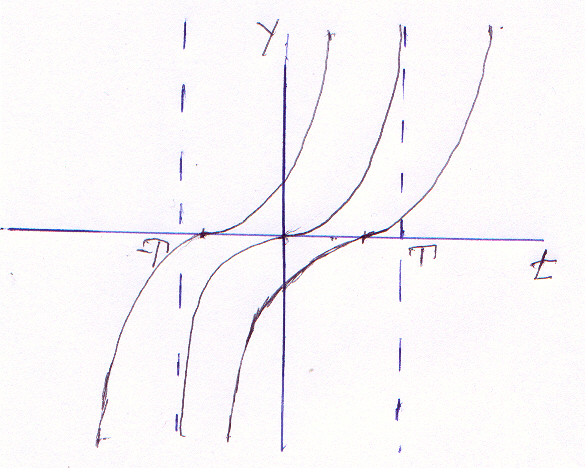
\includegraphics[scale=0.3]{scan11.jpg}	
  \end{figure}
%	\item $$\dot{y} = a(t)y^2 + b(t)y + c(t)$$ 
	
	\item $\forall \epsilon>0$ $\exists d>0$ and $\{d_k\}\leq d$ such that for any increasing $\{\Delta_k\}_{k\geq0}$ such that $\lim\Delta_k$ is finite $\exists K$ $\forall\{x_k\}_{k\geq0}$
	$$|x_{k+1} - \Phi(\Delta_{k+1} - \Delta_k, x_k)|\leq d_k\leq d\quad\forall k\leq K$$
	$\exists p$ and $\exists \{t_k\}$ such that 
	$$|x_k - \Phi(t_k,p)|\leq\epsilon\quad\forall k\geq K$$
	$$\mbox{and }\sum_{k\geq K}|(\Delta_{k+1} - \Delta_k) - (t_{k+1} - t_k)|\leq\epsilon.$$		 
\end{itemize}
\end{frame}
\begin{frame}
\begin{center}
Thank you very much for your attention!
\end{center}
\end{frame}
\end{section}
\end{document}

%\begin{section}{Scans}
%\begin{frame}{Scan1}
%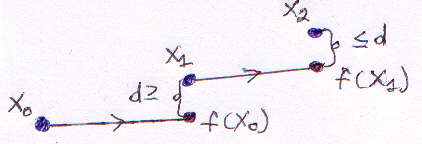
\includegraphics{scan1.jpg}
%\end{frame}
%
%\begin{frame}{Scan2}
%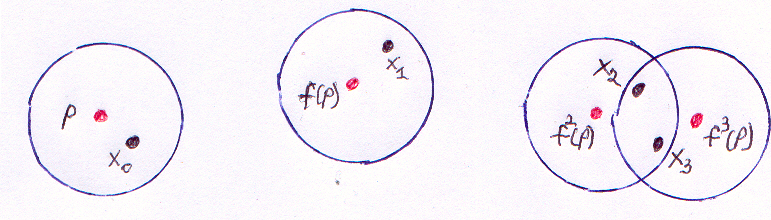
\includegraphics[scale=0.5]{scan2.jpg}
%\end{frame}
%
%\begin{frame}{Scan3}
%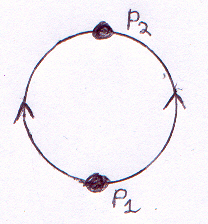
\includegraphics{scan3.jpg}
%\end{frame}
%
%\begin{frame}{Scan4}
%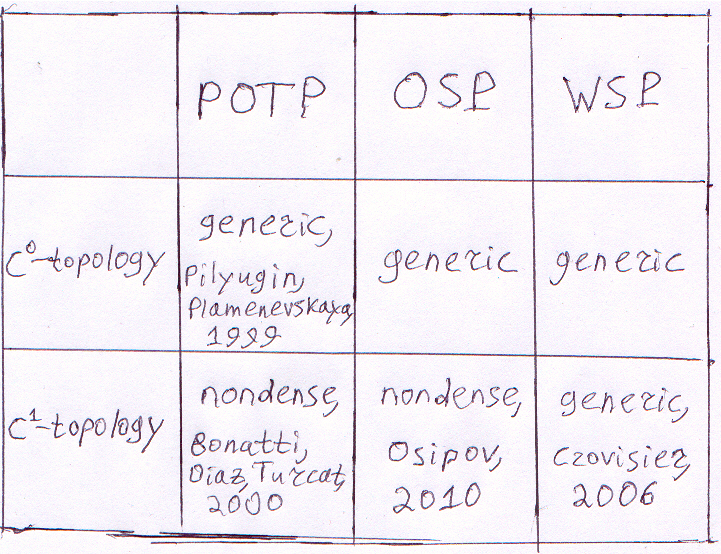
\includegraphics[scale=0.5]{scan4.jpg}
%\end{frame}
%
%\begin{frame}{Scan5}
%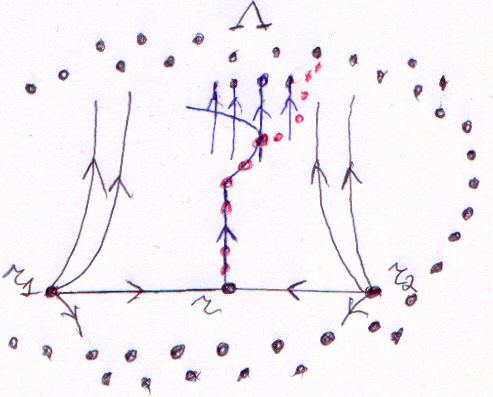
\includegraphics{scan5.jpg}
%\end{frame}
%
%\begin{frame}{Scan6}
%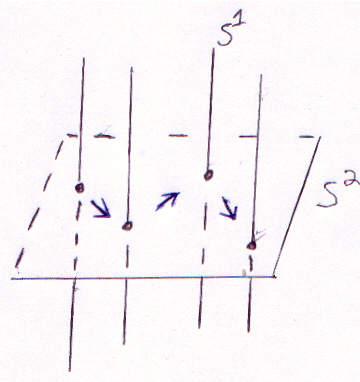
\includegraphics{scan6.jpg}
%\end{frame}
%
%\begin{frame}{Scan7}
%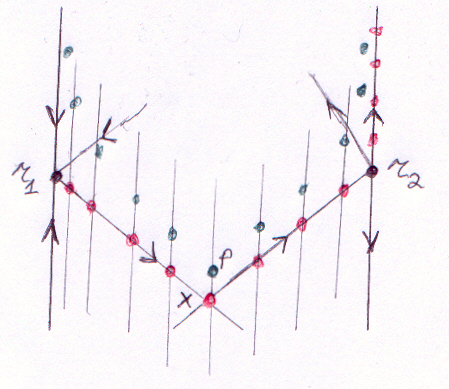
\includegraphics{scan7.jpg}
%\end{frame}
%
%\begin{frame}{Scan8}
%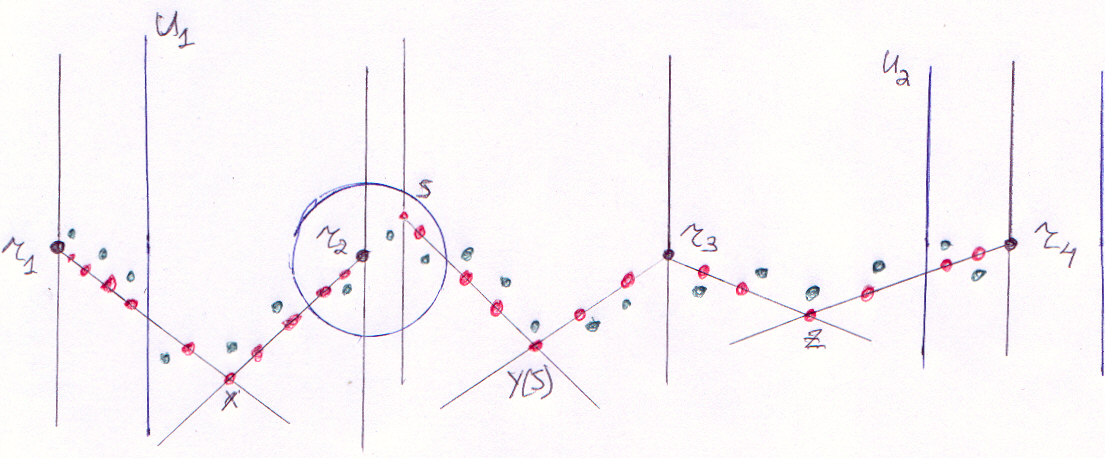
\includegraphics[scale=0.5]{scan8.jpg}
%\end{frame}
%
%\begin{frame}{Scan9}
%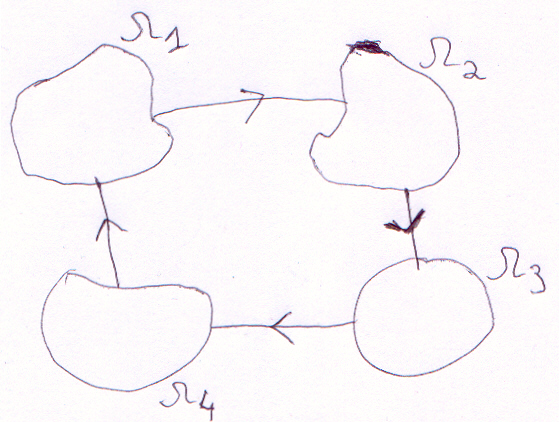
\includegraphics{scan9.jpg}
%\end{frame}
%
%\begin{frame}{Scan10}
%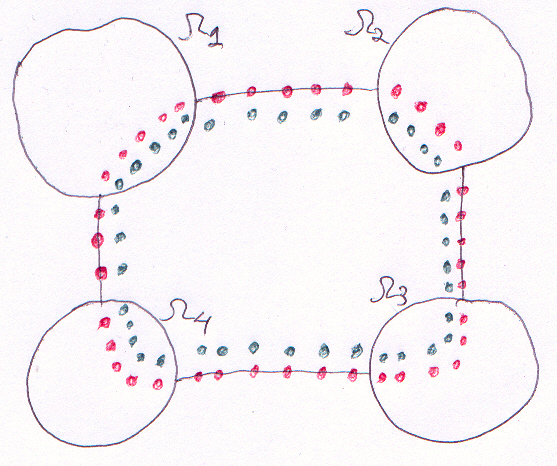
\includegraphics{scan10.jpg}
%\end{frame}
%
%\begin{frame}{Scan11}
%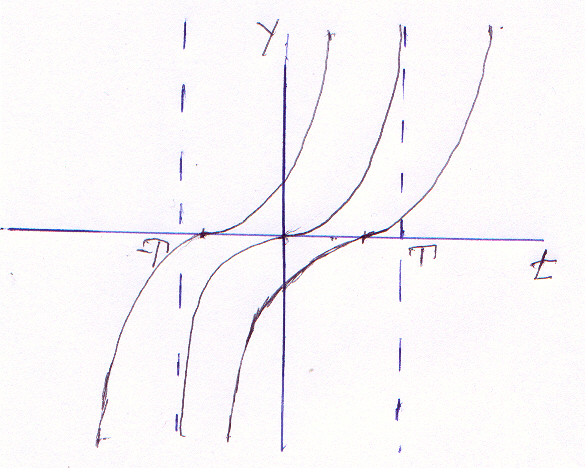
\includegraphics{scan11.jpg}
%\end{frame}
%
%\begin{frame}{Scan12}
%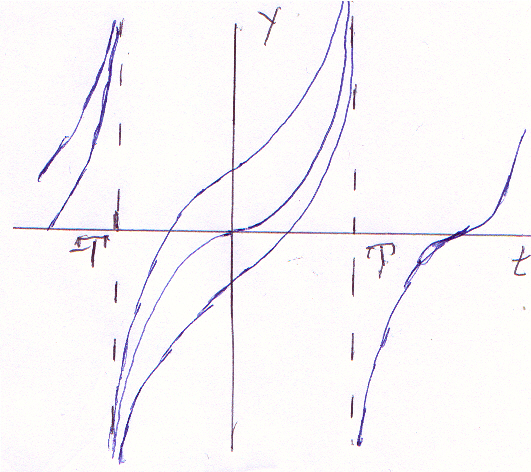
\includegraphics{scan12.jpg}
%\end{frame}
%
%\begin{frame}{Scan13}
%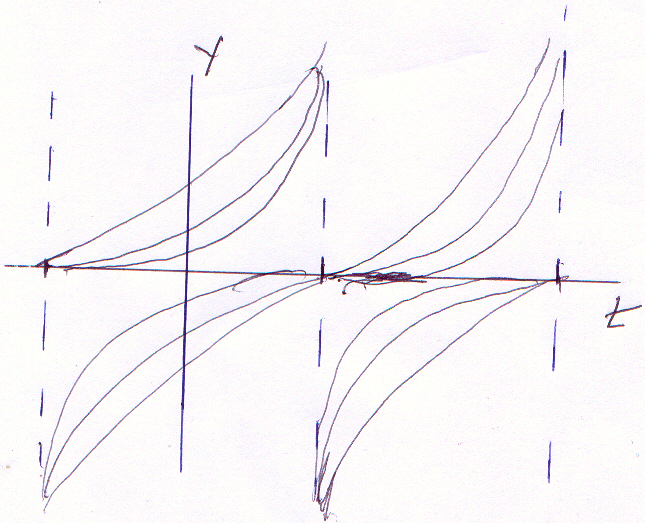
\includegraphics{scan13.jpg}
%\end{frame}
%}